% !TEX root = ../Diplombericht.tex
\subsection{Physikalische Verbindungen}

\subsubsection{Stromversorgung Managementnode}
Der Managementnode wird über den Micro USB Anschluss mit Strom versorgt. Dabei muss darauf geachtet werden, dass ein mindest Strom von 2 Ampere und ein maximaler Strom von 2.5 Ampere fliesst. Zudem wird eine konstante Spannung von 5 Volt benötigt. Deshalb wird ein Netzteil mit einer Leistung von 12.5 Watt benötigt. Das Netzteil wird über eine Stromschiene an das Stromnetz angeschlossen.

\subsubsection{Computenodes}
Die Managementnodes werden über die GPIO Pins 2 und 6 via Jumperkabel mit Strom versorgt (siehe Abbildung ). Da es sich hierbei um eine Anzahl von mindestens 40 Raspberry's handelt ist ein Netzteil mit einer Leistung von 500W vorgesehen. Das Netzteil wird über die Stromschiene an das Stomnetz angeschlossen.

\begin{figure}[H]
\centering
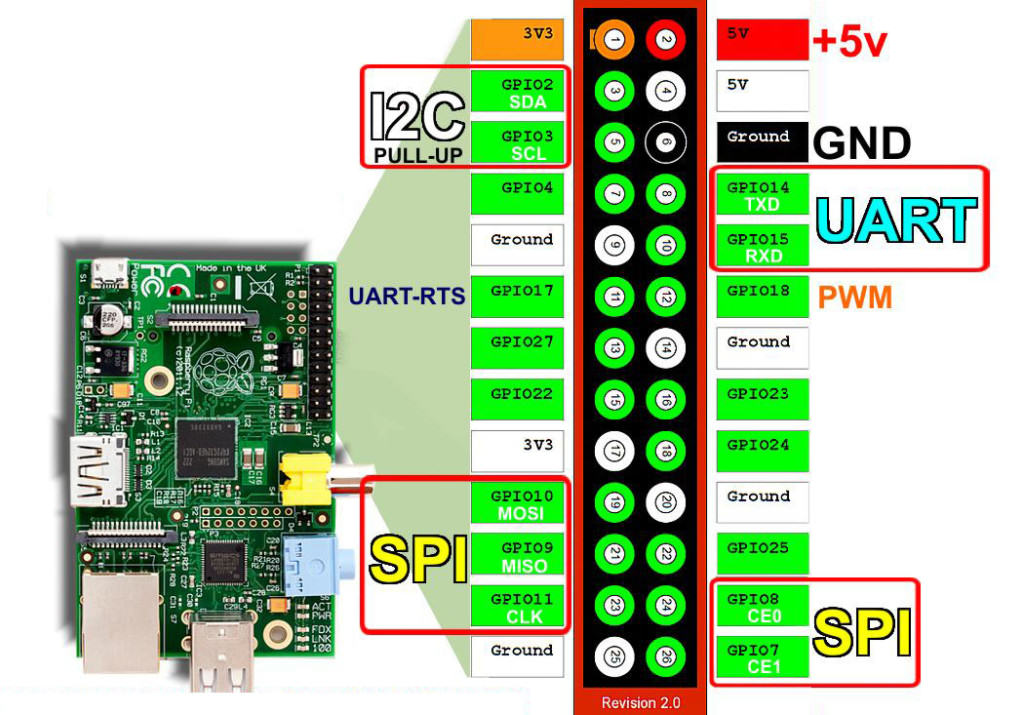
\includegraphics[scale=0.3]{rpi_gpio.jpg}
%\caption{https://developer-blog.net/wp-content/uploads/2013/09/raspberry-pi-rev2-gpio-pinout-1024x715.jpg}
\caption{Eine tolle Abbildung \citep[Quelle:]{https://developer-blog.net/wp-content/uploads/2013/09/raspberry-pi-rev2-gpio-pinout-1024x715.jpg}} 
\label{fig:GPIO Anschlüsse}
\end{figure} 

Quelle: 

\subsubsection{übrige Geräte}
Die übrigen Geräte werdenüber den herkömmlichen Weg mit Strom über eine Stromschiene versorgt.

\subsubsection{Netzwerkverbindungen}
Die folgenden Komponenten sind über den Switch in das lokale Netzwerk eingebunden, die nicht aufgelisteten Geräte werden direkt über Powerline oder WLAN mit dem Router verbunden.
\begin{itemize}
\item Managementnode
\item Computenodes
\item NAS
\end{itemize}


